\documentclass[10pt,twocolumn]{article} 

% use the oxycomps style file
\usepackage{oxycomps}

% read references.bib for the bibtex data
\bibliography{references}

% include metadata in the generated pdf file
\pdfinfo{
    /Title (Comps Proposal Paper)
    /Author (Sammy Sanchez)
}

% set the title and author information
\title{CS COMPS Final Paper}
\author{Sammy Sanchez}
\affiliation{Occidental College}
\email{sanchezs@oxy.edu}

\begin{document}

\maketitle

\section{Problem Context}

For the project that I am doing, I want to make it easier for people that look at sports statistics to visualize the data on graphs to evaluate players. This will be a web app that can help people analyze sports players for fantasy sports that helps them pick the best player of their choice for their chosen stats. The user would be able to select a graph that will visualize the data for playing fantasy basketball. A scatter graph will be created to show where the player's data is at and if other players have similar stats. The stats used for the graph will also be in a chart below the graph to see the data. The user would be able to visualize and evaluate the players that are similar to the chosen player and decide on if they would use the player in fantasy basketball for their team. The user would be able to convert basketball statistics into fantasy points based on the league that they are playing in. Each league has different rules and point totals for each category of stats. An example would be Field Goals Made stat in basketball which would read "FGM = 2 Fantasy Points and TO = -2 Fantasy Points". It will also help users that are interested in sports analytics because of how the app will be a unique way of using stats to visualize a spectrum of where players line up against each other. It will also be different compared to other databases because of the ability to include statistic conversions based on the fantasy league scoring that the user is in. 

There are no fantasy sports apps that analyze stats that the users can put in their fantasy scoring amounts and displays them on different graphs. Fantasy apps currently only display stats on data charts which makes it hard to virtually analyze stats. Being able to visualize stats and players with specific stats chosen will help any fantasy team owner when picking players for their team. The help will come when a fantasy team owner wants to get a player that is similar to another player statistically and it will help generate points for the team over the season. When the best players are chosen by other teams, it gets harder to find players that produce the same amount of fantasy points and this will help target stats that produce points. Being able to group important stats together will help the owner to see how well other players are to a player that does well in the sport. The graph will show a correlation between the stats picked for evaluation, and it will help drive a decision of what player to pick for the team. 

My project would be useful for fantasy players because it will give them an understanding of how different NBA players can be similar statistically which can help a fantasy team accumulate points over the season. It is helpful when the so-called "superstars" are picked in the first couple rounds of a fantasy draft and when there are other players available that have similar statistics to those stars which can help make a positive impact on a user's fantasy team. The impact this project would have on positive players is how the users view these NBA players based on what stats they want to compare and teach them about the impact players have that are not considered stars. 


\section{Technical Background}


For my approach of doing this project, I need to learn how to create a website that can query data from sports stats websites like Sports Reference created by Sean \textcite{sportsReference} and ESPN created by Bill \textcite{espn}. When querying the data it will allow the user to gather those stats from the database websites and create a graph based on the chosen stats. I would have to learn how to create graphs from the gathered data using Python or another coding language that can create graphs. I would need to use an algorithm that can group stats together and make plots on a graph that uses the stats for each player that is being compared. The mathematical equations used would have to be programmed to be implemented when creating the graph based on the stats chosen and might require an algorithm to do it. When the mouse is over the data point, it would have to be programmed to show the player's name on the point. Below the graph would also show the stats used in a chart with other player's names. This could be done by querying to select stats from the sports statistic websites and display them on a chart generated from the query. For selecting stats and the player, I would have to program the website to have drop-down lists that display all the possible options to choose from.

The way people perceived sports data/statistics over the years has changed drastically because of how reliable sports stats have become for professional teams. In an article written by Alyssa \textcite{sportsStats}, she discusses how sports stats were not used as heavily going back to the 1980's and 90's because of subjective gut feelings about players. These were usually biased because of how a coach or front office person would feel about that player. In 2002, she discussed how the Oakland Athletics in the MLB used statistical analysis to created a baseball team of lesser-known players to have a great season and make the playoffs and many people frowned upon the idea of using statistical analysis to make a team that way. Now, sports statics analysis has taken over how fans and employees of these professional teams views players and evaluate them. Many companies have made their own algorithms to track almost all aspects of a respective sport and evaluate the data that they keep track of. 

Another way people have used sports statistics is to predict MVP awards using algorithms and machine learning. In an article written by David \textcite{MVPpredict}, he discusses the way the NBA MVP is awarded based on the people the vote for it and how an AI can predict who is going to win it. The algorithm compares historical data of past MVP winners through two different equations and sees how accurately the AI predicts the MVP. It used MAE (Mean Absolute Error) and R² (coefficient of determination) to evaluate the MVP as seen in Figure 1. The experiments that were used were to see if it correctly identified the MVP for a specific year and would calculate the accuracy of guessing the MVP correctly. 

\begin{figure}
    \centering
    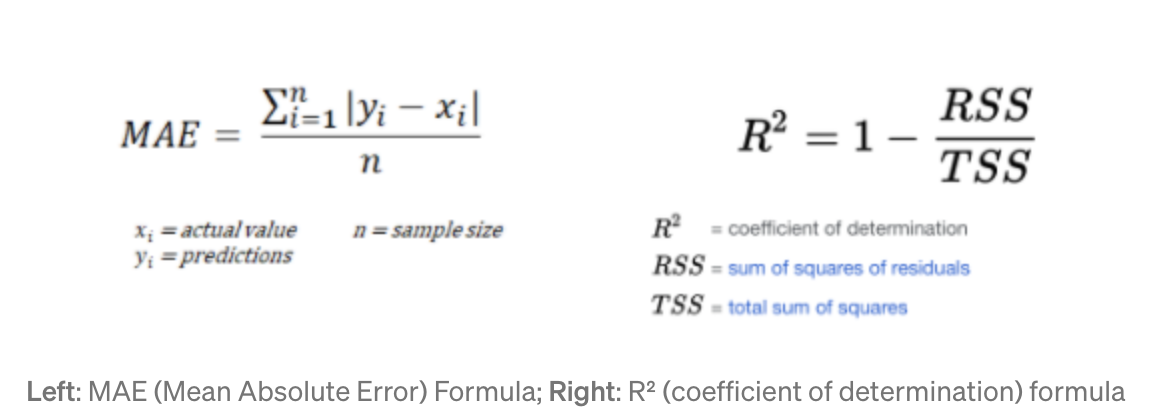
\includegraphics[width=.95\linewidth]{stats.png}
    \caption{
        MAE and R²
    }
    \label{fig:second-page-1}
\end{figure}


\section{Prior Work}

The prior work that has been done is a website called "NBA Player Performance and Scouting Explorer" and the website is created by \textcite{dash}.
It is designed to be used as a way to view and group NBA players with stats on graphs. One of the graphs uses body weight and height as a way to group players with higher physicality or you can group the player strictly off statistics. The players are grouped in the graph based on their position in basketball and a player is selected to be compared to with a chart listed below the graph with the stats. It allows the user to also group players based on the custom stats they choose to evaluate players. Another option to use in this app is how stats picked are grouped together and groups are made for players that are similar to those stats. It is something similar to what I want to do with my project, but in this app, the stats that can be used are limited and I want to expand it with more. It is also only used for basketball players and I would expand it to other sports like baseball and football. In Figure 2, it shows the visualization of Steph Curry compared to other players in the NBA that have a similar physicality to him, but also shows how statistical data compared to him as well. The inspiration for this website can be to find good NBA players and be unbiased using their app. As a user, they can pick their favorite player and compare them to other players using stats or physicality of the chosen player and the results will be unbiased. Biases in sports are very common because of many factors like the home team, not liking a player because of their persona and etc.

\begin{figure}
    \centering
    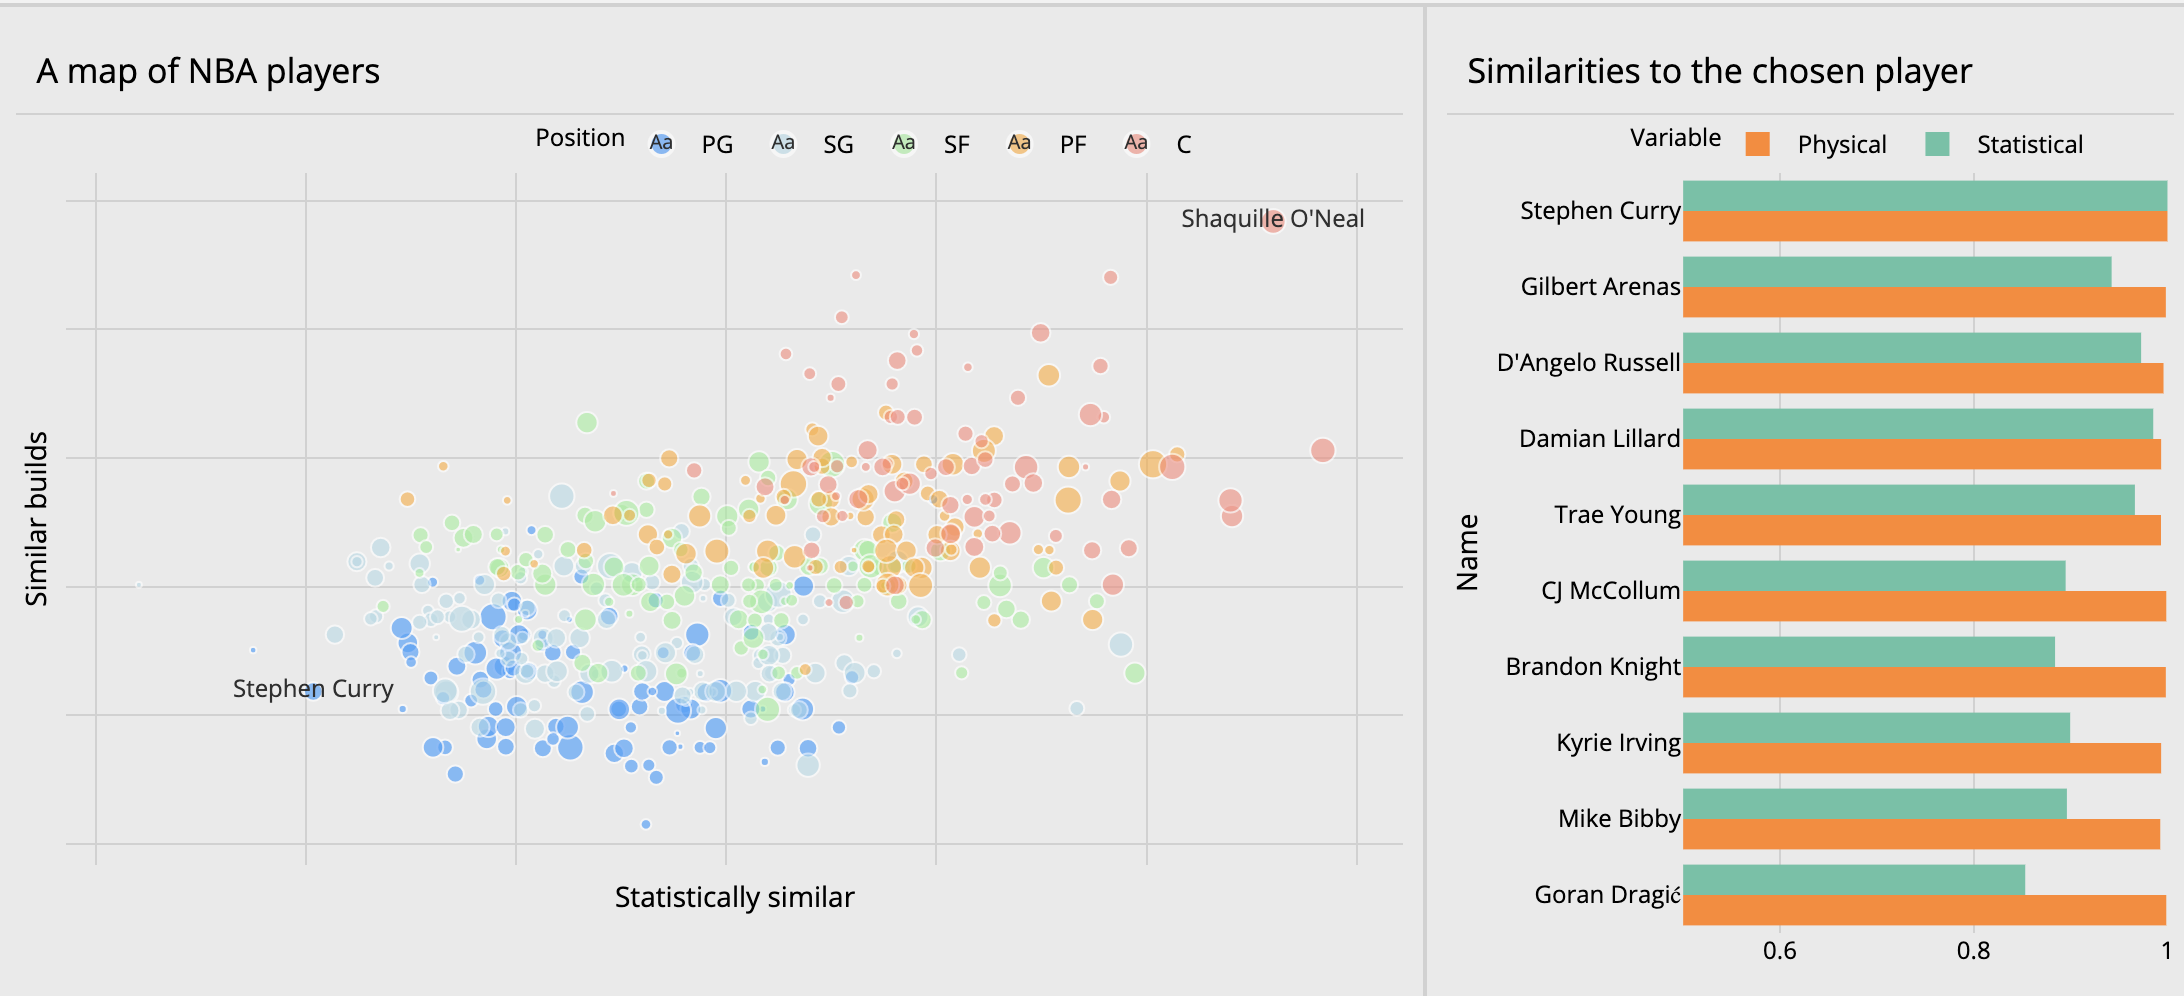
\includegraphics[width=.98\linewidth]{Steph_Comparisons.png}
    \caption{
        Steph Curry's Physical Comparison to other Players in the NBA 
    }
    \label{fig:second-page}
\end{figure}

Another work that is similar to my project is the website StatMuse created by Eli 
\textcite{statmuse}.
The user can use key words to look up stats for a team or players across all sports in America. It displays the stats the user was looking for in a chart after the website finds the specific stats. Examples of specific stats can be a specific player vs a team in their career, most point in a game in a specific year and much more. The website also has fantasy sport projections that users can ask the website. It will display a projection number in a chart for the player they want to know about. Compared to what I want to do, I would simplify this by not using keywords to look up stats and display graphs of the data that the user want to visualize. In Figure 3, when looking up stats in Statmuse, you have to use keywords and the words used are "steph curry playoff win-loss record". With this, it shows the playoff record of Steph Curry's whole basketball career and the overall stats for those playoff games for each year he has gone to the playoffs. The inspiration for the Statmuse website comes from analysts and people that watch/engage in sports because of how these people want to find specific stats of players and teams that can be meaningful. An example would be finding out if a player does good in elimination games and can be evaluated based on those stats which are negative, neutral, or positive. 

\begin{figure}
    \centering
    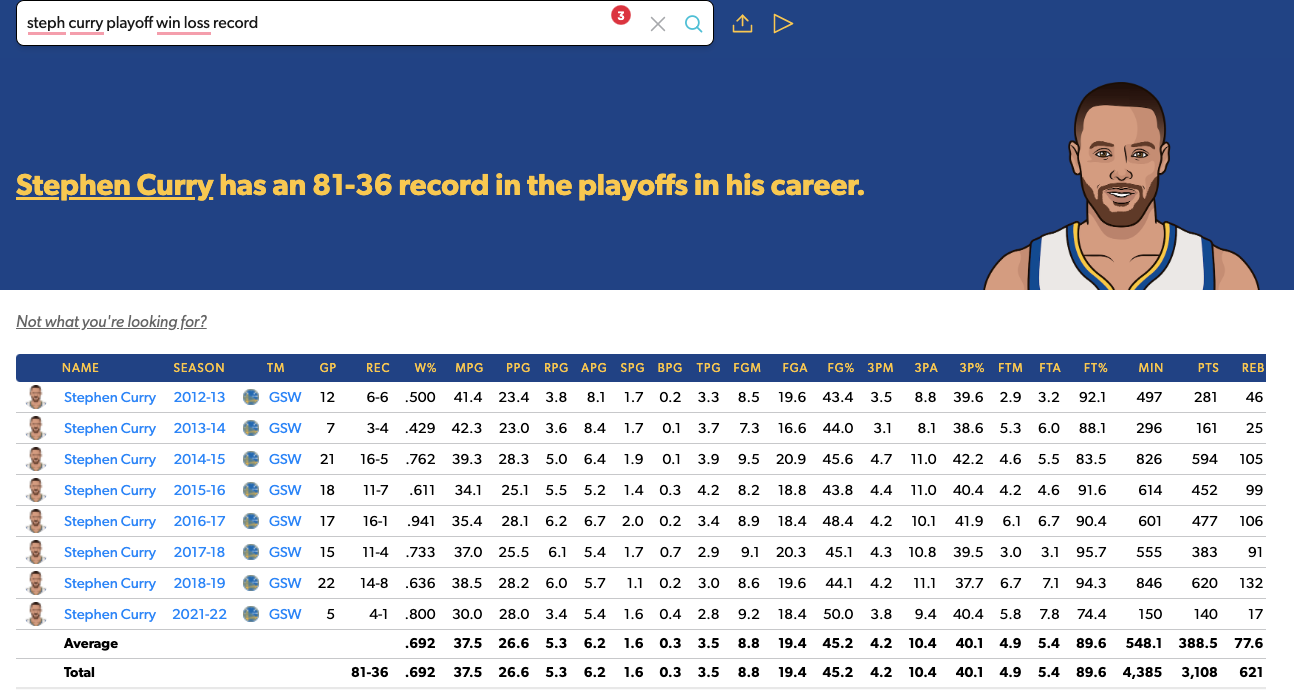
\includegraphics[width=.98\linewidth]{StatsMuse_Curry.png}
    \caption{
        Steph Curry's Playoff W/L Record with Stats
    }
    \label{fig:second-page-2}
\end{figure}

\section{Methods}

What I planned on doing for collecting the NBA stats for my project would be to query them from sports stats databases like \url{https://www.basketball-reference.com/}. I would have had to make an algorithm to pull these stats from the website based on what player the user chooses like "Stephen Curry" or "Lebron James" and what stats they specifically choose to evaluate the players and make comparisons. If the algorithm to pull or query the data from the database website does not work, I would find a way to add all the total stats to a CSV file which would make it easy to query data. Since the data is typically shown in a chart, I think it would be easy to copy that data in a format that would match a CSV file. When creating an algorithm to pull the data from basketball-reference, it did not work, but there was an option to add all the data to a CSV file manually.

I would extract the statistical data from the previous regular season, so 2021-22 season by using an option the website had. It gave me the option to convert the data to CSV file format, so I had to copy and paste the data and then add the data to a CSV file. 

I planned on querying the data that the user chooses for fantasy basketball, for example, total points and rebounds, and then having a datasheet of players and those specific stats. Then, the algorithm would look at the stats in the data sheet and calculate points of data on the graph, and set the points with the player chosen highlighted. When a user drags the mouse over a point of data, it says the name of the player. This was not used because of how I needed fantasy point values and lots of user input for \textcite{poltlyInfo} which just programs graphs without the user checking boxes of what goes on each axis and etc. 

For how the statistical data is going to be calculated and shown on a graph/chart, I needed to create an algorithm using python to create and display data on a graph and show the stats used on a chart below. Python has lots of libraries like pandas that would make it easy to calculate data and put data on different types of graphs. Python also has something called \textcite{poltlyInfo} which helps users code graphs from data. I could build a web app from using \textcite{dashInfo} which is a part of Plotly using the data that I get from the database website. 

I also had to figure out a way to convert the statistics into fantasy points. The way I would do this is to create a program to read the CSV file data from the database website and convert each category to fantasy points. I would have to allow user input for what each statistic is worth in a fantasy league. After getting the user input, I would make the program calculate the new fantasy stats for every player and save it onto another CSV file for use of the Plotly python program. 

The datasets of a survey of potential users who might want to use my app for fantasy to look for the value of players was useful for my project methods because of what the users want to see when evaluating different players. I created a form for fantasy basketball users and discuss what they are looking for when drafting players for their fantasy teams. I asked them what stats they look for when picking players, what positions they prioritize in fantasy, and how they would use data given to them based on looking at a visualization of sports statistics. I asked them about their strategies for drafting players and if they do it based on personal opinions about the player. An example of personal opinion would be like wanting a "star" player in the NBA on the fantasy team or drafting an underrated player based on statistical data. The survey was used for me to code the different graphs and plots for the project.

The data I am going to show to the fantasy users is based on the stats or graphs they choose to compare the players. They will use this information to influence their draft picks and evaluate the player's value. This graph produced shows the user players that are statistically similar to the player of their choice and the stats that they also want to compare. The data shown would be a graph with different points of data that represents a player in the NBA and below the graph would be a chart of the data to see what was used to calculate the graph's data points. The graph's data will be calculated using the stats converted to fantasy points. For example, if the user picks 3-pointers made, field goals made and assists as the data to be compared, it will show the user a graph of the player chosen like Ja Morant compared to other players with stats that are similar and create many points of data on the graph. It will look roughly like Figure 2, but the graph is more simplistic and gives information for what point of data represent a certain player and shows the chart of data used to compare. The graph I programmed to show different categories of fantasy points scored on a stacked bar graph with negative points being on the negative y-axis and positive points being on the positive y-axis. The users can select and deselect which specific categories they want to compare for different players. Plotly was used to program the graph and the data was used from the CSV file of the converted fantasy points data. It is aimed to help the user know if a player is scoring many fantasy points from specific or many categories and that they could compare players visually on the bar graph.

Another graph that was created in the project showed the user what total positive and total negative fantasy points are shown and it was also on a stack bar plot. The player's names are on the x-axis in alphabetical order and the user can also click on the categories to select and deselect the two stats shown. It is aimed to help the user know if a player is scoring many positive fantasy points or if the player scored many negative fantasy points and that it is impacting the fantasy point total for the player.

Another graph that was created in the project showed the user what total positive and total negative fantasy points are shown and it was also on a stack bar plot. The player's names are on the x-axis in alphabetical order and the user can also click on the categories to select and deselect the two stats shown. It is aimed to help the user know if a player is scoring many positive fantasy points or if the player scored many negative fantasy points and that it is impacting the fantasy point total for the player.

A chart was used in the project's web app to display all of the converted fantasy points total. The user could use this to quickly see the total points in chart form if they decide they want to draft or pick up the player for their fantasy team. 

A graph that was made in the web app showed the true total of points for Field Goals and Free Throws of a player. Field goal attempts and Free Throw attempts are typically negative points in Fantasy Basketball and I programmed a calculation to see if there are negative or positive points for those two categories. It was also displayed on a stacked bar graph to show users if a player is gaining or losing fantasy points from those categories. The goal is to help the user with the visualization of these stats.

A scatter plot used in the web app showed the user the total fantasy points scored to make it easier to differentiate between different players. The graph was also sorted in a different color per position of the player to let the user know what position they are in because of the fantasy limit of having a certain amount of players per position. 

Another scatter plot used in the web app showed the user the total fantasy points scored on the y-axis and the total points scored throughout the season on the y-axis. The goal of this graph is to show the user the fantasy players that score the most points in basketball and if it corresponds or correlates to the total fantasy points being scored.

All of the graphs or plots I programmed for the web app were influenced by fantasy user feedback on what they look for when picking up or drafting fantasy basketball players. I tried to take into account of adding a search bar for looking up specific players, but this approach was not doable. I attempted to program that feature, but I was unable to successfully do it even though I had some feedback from potential users that said it would be useful. 


\section{Evaluation}

To do a mock fantasy draft as a way to test the potential of the project would be to make the fantasy users pick a player from each position that they like and use the project to do the comparisons of stats for each of those players. They would write down 5 other NBA players that are statistically similar in a chart under those players just in case they get chosen in the draft and have backup options. While doing a mock fantasy draft, the users can see if they can get the players that they wrote down and simulate a season for fantasy to see if the players chosen performed to their expectations based on the project. I would get feedback from the users to see what their opinion was on drafting certain players that they picked from the graph of the project.  

To evaluate my project, I would do mock fantasy drafts and simulate the fantasy seasons based on the 2021-22 season to see results using my project to pick players. My project would be used to find a player with the specific stats that the user wants to take advantage of when other similar players are taken off the board like a superstar in the NBA like Lebron James. The fantasy season would be simulated to see what place the user got in fantasy and to see if the players that were recommended had a positive impact on their team. The list of players that the user produced from the project would be used to influence how the user drafts players in the mock draft. Since they will have many options for each position that the player user has to fill for their team, they can find players that were statistically similar to the player that they like or are considered a "star" in the league. Results from a simulated fantasy season will allow the user to see the impact of the players chosen from the project based on how many individual fantasy points were scored. I would get feedback from the users to see if they agreed with what the project produced when they used it and if they thought the project was accurate in evaluating the players. It would be based on the user's opinion because NBA players picked in fantasy drafts can underperform and users would not like that because of how there will be a lack of fantasy points. I will ask them if the visualization was easy to follow and comprehend when evaluating the player and other players statically. I would ask if looking at the chart of the stats was more effective than looking at the visualization on the graph and vice versa. Another question would be if the project worked well with both the visualization and the chart for reference or if one was better than the other at evaluating players. Asking the user what statistics they prioritize in fantasy is key because fantasy sports are all about scoring fantasy points and not losing points based on specific stats like turnovers and field goal attempts. I also considered if the fantasy user preferred looking at charts or looking at graphs and plots when comparing stats.

The source I would have used to evaluate the player chosen in the draft would be using the Yahoo Fantasy Draft Analysis \cite{fantasy}. This website shows you data of the average pick that users picked the player, what average round they were selected, and the percentage drafted in all Yahoo fantasy sports leagues. These statistics are used to see how popular draft picks are and with it, you can click on the player and it will show the NBA stats and fantasy stats points and the ranking of the player. The user can use this website to evaluate the players they chose and can give feedback on whether it was a good pick, neutral pick, or bad pick. They will give feedback on if they thought the project misdirected them or helped them with their picks. Figure 4 shows the top 5 players picked in fantasy sports for the 2021-22 NBA season. The highlighted blue box column allows a user to look at the fantasy sports statistics and see the rankings of the players for the year. 

\begin{figure}
    \centering
    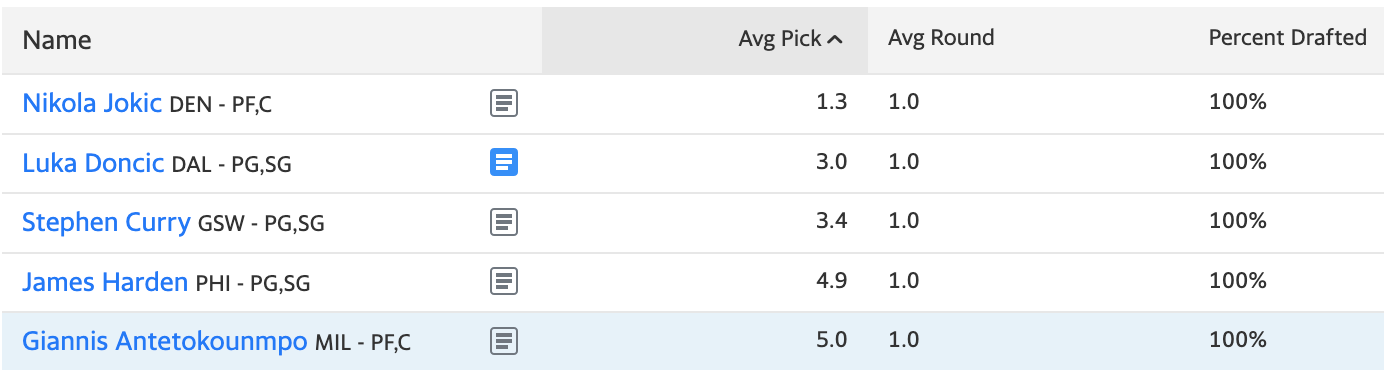
\includegraphics[width=.98\linewidth]{top5.png}
    \caption{
        Yahoo Fantasy Draft Analysis Top 5 Picks 2021-22 Season
    }
    \label{fig:second-page-4}
\end{figure}

I considered using Yahoo Fantasy Draft Analysis as a part of the evaluation but ended up not using it for evaluations. The reason that I ended up not using this metric was because it only gave an analysis of the player and ended up having little to do with the drafting. The draft analysis just shows what their computer model predicts what the player is going to score and would not have been useful to how I evaluate my project. I would rather the user do a mock fantasy draft and tell me about their experience using the project compared to the players they drafted being evaluated for fantasy points impact. 

The source that I used for evaluation is the ESPN mock draft website \cite{fantasyDraft}. This would allow a user to test the project by doing a mock draft and seeing what players they can pick for their team. Using my project would help influence the users to pick players that are statistically similar to a player that was already chosen. Then the user can join a fantasy league and simulate the previous basketball season to see how well the team performed with the players based on the project. To be able to evaluate how well the project worked, I would ask them if drafting the players was positive or negative based on what the graph produced when comparing NBA players and their stats. A question would be what kind of stats they compared and if they would change them if something did not work out. I would also ask them what kinds of fantasy league it is like head-to-head, most points overall, or categories of stats and which one type of league would best benefit from using the project. For this draft simulation, I would ask the users what strategies they use for fantasy drafts in general and what they would do differently using my project for influencing their decisions. Figure 5 shows what kinds of mock drafts a fantasy player can do with different league rules of how scoring is tallied, which can change how the project is evaluated. If the users can spot differences in choosing players in different types of fantasy leagues, I can evaluate which fantasy league would be the best option to use my project for. Also, I would be able to evaluate if the visualization of the graphs shown helped the users compare players and influenced them to draft differently.

\begin{figure}
    \centering
    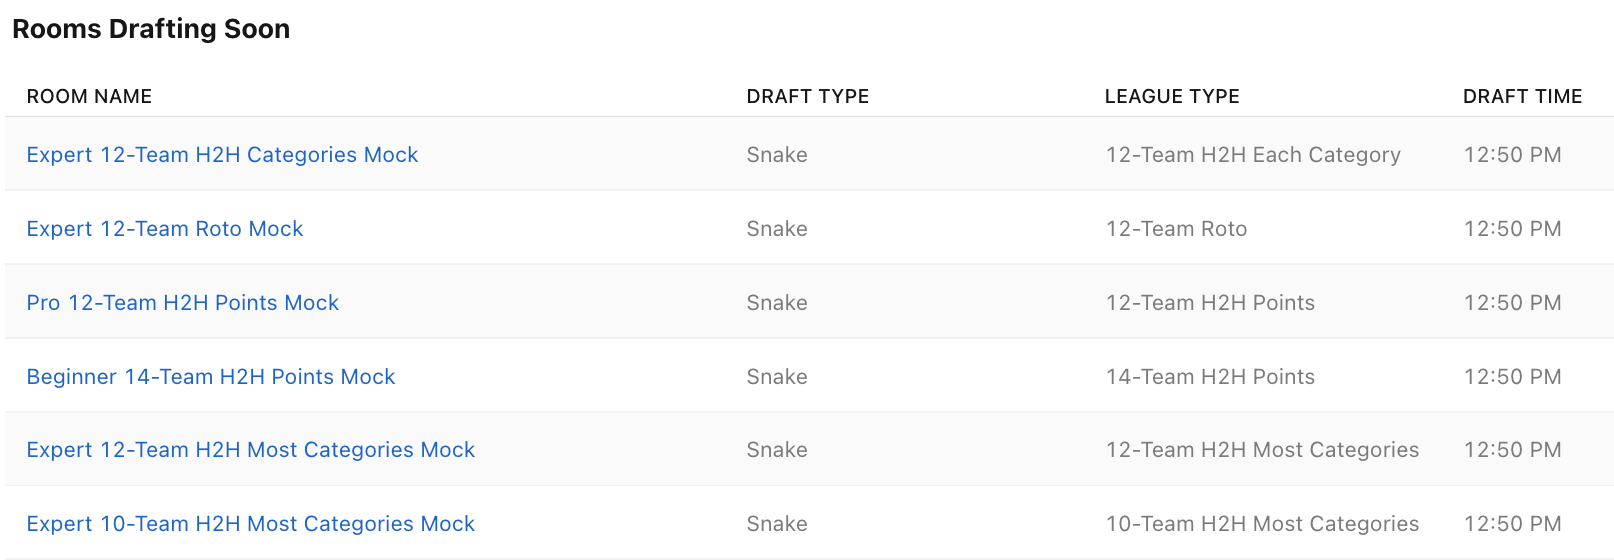
\includegraphics[width=.98\linewidth]{mockdraft.png}
    \caption{
        Different Types of Fantasy League for Mock Draft
    }
    \label{fig:second-page-5}
\end{figure}

Overall, I gathered all the information I received to evaluate how well my project would influence a fantasy player to use it to help draft a team. Evaluating the reactions to using my project from the user standpoint is a big way to see if the project positively or negatively helped their team or if they thought the project was useful or not. I would calculate different variables of the percentage of users satisfied using the project if the team did well in fantasy and if the players chosen were a good choice overall. I can also calculate the percentage of users satisfied with the project itself and use it to compare players and take feedback to improve the project and pinpoint issues with using it. 

\section{Results and Discussion}
For the results of the mock draft, there were positives and negatives about the use of this project to help fantasy users draft players using statistic visualization. 

The goals of this app are to let a user would be able to select a graph that will visualize the data for playing fantasy basketball. The user would be able to convert basketball statistics into fantasy points which would be graphed or plotted for data visualization to help them compare players. Using the users utilized the ESPN Fantasy Mock Draft\cite{fantasyDraft} website for the mock drafts and used the web app as a way to compare players and visualize their stats, it was mostly hard for them to use the web app and draft a player within the time period of drafting. Some users complained that not being able to search for a player was a big reason why it was hard. With this being a negative issue, it made the web app useful for data visualization and comparing players when having an unlimited amount of time instead of being rushed when drafting in fantasy basketball.

For the results on if drafting the players was positive or negative based on what the graphs produced when comparing NBA players and their fantasy stats, I would say there were more positive than negative reviews. More than half said that it was easy to see what players scored more than other players, especially for the graph that broke down each category of points scored per player. Some users also mention viewing the negative and positive statistics graph influenced them to not draft a player because of the negative fantasy points they produced. The reason for this result was because of how the stacked bar graph showed the differences between each player and how many fantasy points they have scored from each category. The positive result also shows how visualization helped the users pick one player over the other based on the graph showing their impact on scoring. The more negative users said it was hard to compare if they could not select certain players to compare when they see all the players listed. Not having a side-by-side view of the selected players made it difficult to compare. The reason for this negative result is because of the lack of searching and grouping player names in the web app. Another result could be from the user preferring to look at charts of data instead of graphed data and the web app not providing a way to select players' stats on the graphs/charts to highlight their stats.

For results on what kind of stats the users compared and if it was impactful on their choice of drafting, many users claimed that they mostly looked at total fantasy points scored while some users broke down what a player scores for certain categories using one of the stack bar graphs which gave them a new way of viewing how a player scores their fantasy points. I think the result of the users just looking at the total fantasy points scored per player is common because that is what fantasy users want on their team; a guy that can score lots of fantasy points. The fantasy users that broke down the points scored for certain categories of the fantasy points influenced them to think differently about how that player scores fantasy points and if they gain more points from a certain category of stats. 

For the user strategy they would use for fantasy drafts in general and what they would do differently using my project for influencing their decisions, some users said they would look at how the fantasy points are scored between the different categories of scored points. Some users said they would look at the negative fantasy points and how they impact a player's total fantasy points. Some users also claimed it might help them find hidden talent/role players that could score many points for their fantasy team. This result accomplishes one of the goals of how this app could help the user draft players that are not considered stars. 

For evaluating the reaction result to using my project from the user standpoint I got mixed reviews on whether to use it for the fantasy basketball drafting process. Using a 1-5 scale with 1 being not helpful/useful to 5 being most helpful/useful, almost half the users had said it was a negative experience (2.5 or lower) when using my web app while the other half had a positive experience (2.5 or higher). The number of users that were influenced with drafting a player based on using my web app was about the same as to the web app being helpful. These results could have occurred because of the positive users using the graphs for visualization as a new way to see players and their fantasy worth. The negative results could have come from the web app being annoying to use and their preference for just looking at charts instead of graphs and manually finding the players. 

Overall, the project had mixed results for fantasy drafting, but one portion of feedback stood out. One user suggested that the web app would be better for doing research on impactful fantasy players before a draft and taking time to compare players. As a result of this feedback, the web app could be used to scout players that will have an impact on fantasy teams and allow the user to compare and visualize players' stats before and after a draft to trade for a high-scoring player. For the goal of helping a fantasy user draft a better team using stats visualization, I think the result can point to the web app being useful for that, but only if the user uses it to find players that make an impact before the draft and after the trade to conduct trades. I think my project goal of helping the fantasy user use visualization to find players that are not considered "superstars" that make a positive impact on their fantasy team based on some feedback that the user noticed role players with high fantasy scoring.  

\section{Ethical Considerations}
Some ethical issues can occur when my project is used to degrade players based on their statistics, especially if the stats are viewed as negative. My people use social media to spread this information and sometimes cause people to go after the sports player on social media with harassing comments. to combat this issue would be to disclaim to the users about not judging the player based on the stats they chose because those stats do not fully make the player. 

In an article written by Jack Bowen about Fantasy Sports and its impact on society \cite{fantasyEthics}, he discusses how fantasy sports consumption can lead to unethical ways we treat sports players. He makes points about how players who miss games or score low in fantasy sports can lead to fantasy users leads to unethical treatment because of how they do not contribute to a fantasy team. Athletes are treated as fantasy players whose only purpose is to score fantasy points and how it impacts a fantasy user's team. A quote Bowen uses that describes fantasy sports and player treatment is: "Fantasy Sports has the potential to create a moral habit in its participants in which they reflect on these people—the athletes—in a way antithetical to how we otherwise think best" \cite{fantasyEthics}. An ethical concern for my project is that it would be used for fantasy sports that impact the way fantasy users perceive and treat sports athletes if they do not score enough fantasy points. It can create a bias towards players who score more in fantasy sports and leave other players to not be considered as good fantasy players. Based on how a user looks at the data, that is how bias can be created especially if the user values their own opinion over statistical data.

Some ethical concerns with my project might be how money is involved in fantasy sports and my project can influence people to bet and potentially lose money if they use my project's outcome to draft players. If a user is deadset on just using the project and it influenced them to bet or wage their money on thinking the project will get them a guaranteed win, it can be unethical because that is not what the project is for and it is only to help a user evaluate players to potentially draft in fantasy. To combat this issue would be to disclaim that this project is not for betting and should be used as a guide to evaluate players and rely on their own instincts when making decisions. 

Another part of the Bowen article is about how fantasy sports can connect to online gambling with websites like DraftKings. A quote that Bowen uses is "There’s no doubt it requires some skill to play Fantasy Sports well(an important caveat) but many who are prone to the addictive nature of gambling participate in Fantasy Sports rationalizing it as being 'just a game' or, 'a way to connect with my love of sports.'"\cite{fantasyEthics} Gambling is used in fantasy sports when fantasy users decide to make or join a league. Typically, a league has a buy-in price to make the season have stakes of winning money if they happen to win the entire league. An ethical issue that can come out of this is how my project can be used to feed a person's gambling habit thinking that they are going to draft the best fantasy basketball players in the league. 

Issues of bias from my project can be from how fantasy users view the data provided to them on the graphs. The data visualization aspect of my project can lead to bias because of how visualization has the potential to show the statistics in a misleading way. In a research paper about visualization literacy and biases written by Hamid Mansoor and Lane Harrison, they claim that: "The attraction bias occurs when a viewer’s choice of two options is influenced by an irrelevant third choice, i.e. a choice that is clearly inferior to both the original ones. To test the extent to which the attraction bias manifests in visualizations, they conducted a user study with tables (as a baseline) and scatterplots. The results of this study indicated that data visualizations are also prone to this bias, causing people to make errors in judgement."\cite{visualizationBias} They state that users who view visualization can make judgment errors on the data that is presented which can apply to my project as this is a bias issue. Data from the visualizations in my project could potentially lead to bias based on the user that views the data and how they interpret it. Confirmation bias and be used to prove to the user that a player is better than another based on the graph that is shown for fantasy points scoring, especially for the categories of how fantasy points are scored.




\printbibliography 

\end{document}